\documentclass[11pt]{article}
\usepackage{amsmath,amssymb,xspace,epsfig}
\usepackage{algorithm}
\usepackage{algpseudocode}
\usepackage{algorithmicx}
\usepackage{graphicx}
\usepackage{subfigure}

\graphicspath{{plots/}}


\textwidth 6.5in \textheight 9.05in \oddsidemargin 0.0in
\evensidemargin 0.0in \topmargin -0.55in
\addtolength{\textwidth}{2.5mm} \addtolength{\columnsep}{2mm}

\title{Report of assignment 1}
\author{Haoyang Zhang, Qi Wu, Shengjie Li}


\begin{document}
\maketitle

	\section*{Questions}
	\begin{enumerate}
		\item what do you expect to happen if an IF neuron is constantly fed a very low input current? An LIF neuron?
		
		IF: Because the neuron continually integrates input, its membrane potential $V$ will constantly grow up. Finally, $V$ will reach the threshold $V_{threshold}$ and the neuron will fire.
		
		LIF: The potential is dominated by current "leak" which tend to set the voltage to 0. So, the voltage will increase from $-65$ to $0$ at the begin. Then, the input will be counteracted by "leak" and voltage will converge to $0$.
		
		\item what do you expect to happen if an IF neuron is constantly fed a large input current? An LIF neuron?
			
		IF: Neuron will fire and reset its membrane potential in a very high frequency.
		
		LIF: Neuron will have a similar performance as IF. Because the membrane potential is dominated by input current, and the current "leak" can not counteract the input.
		
		\item What are the limitations of an LIF neuron?
			
		The LIF neuron can't handle large input. In this situation, LIF will be similar with IF that the firing rate is linear correlation with input current. See \ref{fig:Fig1.sub.I}
		
			\begin{figure}[htb]
			\centering
			\subfigure[Low input]{
			\label{fig:Fig1.sub.L}
			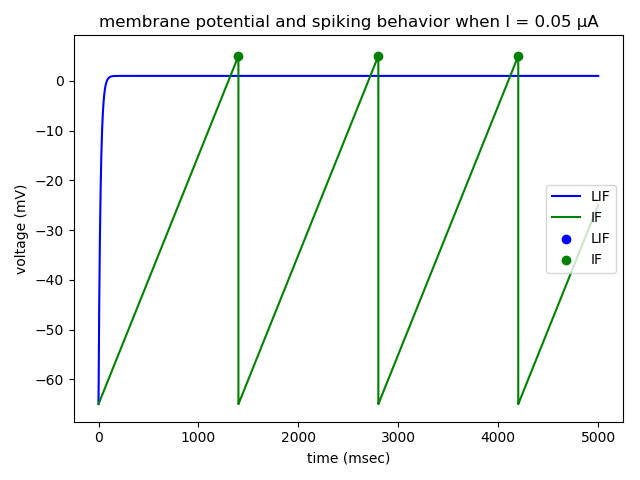
\includegraphics[scale=0.2]{plot_question_1.png}}
			\subfigure[High input]{
			\label{fig:Fig1.sub.H}
			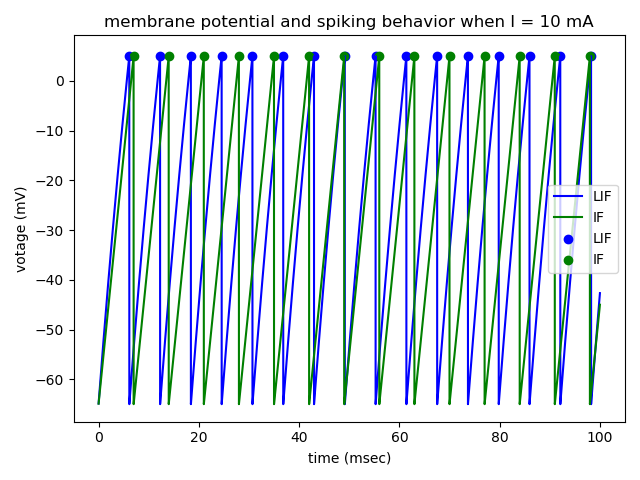
\includegraphics[scale=0.2]{plot_question_2.png}}
			\subfigure[Increasing input]{
			\label{fig:Fig1.sub.I}
			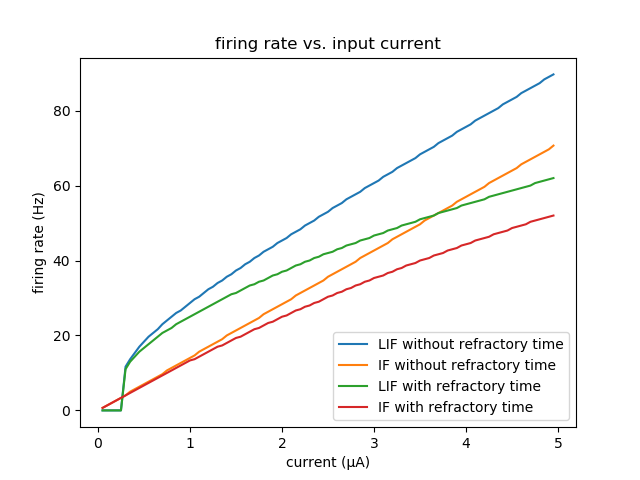
\includegraphics[scale=0.2]{plot_question_3.png}}
			\caption{LIF and IF}
			\end{figure}
		
	\end{enumerate}
	
	\section*{Programing}
	\begin{enumerate}
		\item Simulate an LIF neuron with different input currents and plot the membrane potential, showing (a) potential decay over time and (b) spiking behavior.

		See \ref{fig:Fig2.sub.voltage}.
		
		\item Plot the firing rate as a function of the input current.
		
		See \ref{fig:Fig2.sub.voltage}.
		
		\begin{figure}[ht]
			\centering
			\subfigure[Potential]{
			\label{fig:Fig2.sub.voltage}
			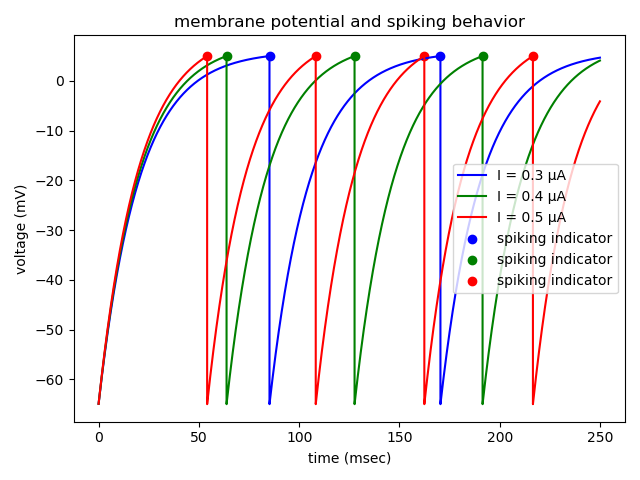
\includegraphics[scale=0.3]{plot_programming_1.png}}
			\subfigure[Firing rate]{
			\label{fig:Fig2.sub.fire_rate}
			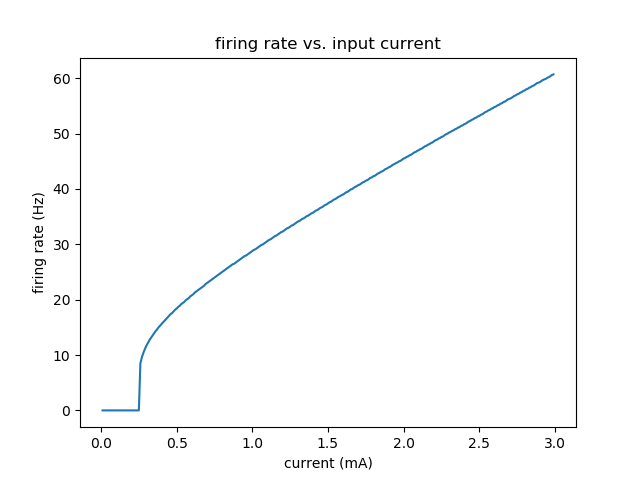
\includegraphics[scale=0.3]{plot_programming_2.png}}
			\caption{LIF and IF}
		\end{figure}
		
		\item What happens to the firing rate as you continue to increase the input current? Why?
		
		See \ref{fig:Fig2.sub.fire_rate}, when the current is small, the firing rate will increase steeply as increasing current. This is because ?. As input current increasing, because the potential will be reseted to $V_{rest}$ after firing, $R_mI$ will be far larger than $V$. In this case, the potential will be dominated by input current, and the firing rate will be linear correlation with input current.
		
		\item Simulate a neuron using the Izhikevich model.
		
		See \ref{fig:Fig3.sub.Izh}.
		\item Simulate a neuron using the Hodgkin-Huxley model.
		
		See \ref{fig:Fig3.sub.H-H}.
		\begin{figure}[ht]
			\centering
			\subfigure[Izhikevich]{
			\label{fig:Fig3.sub.Izh}
			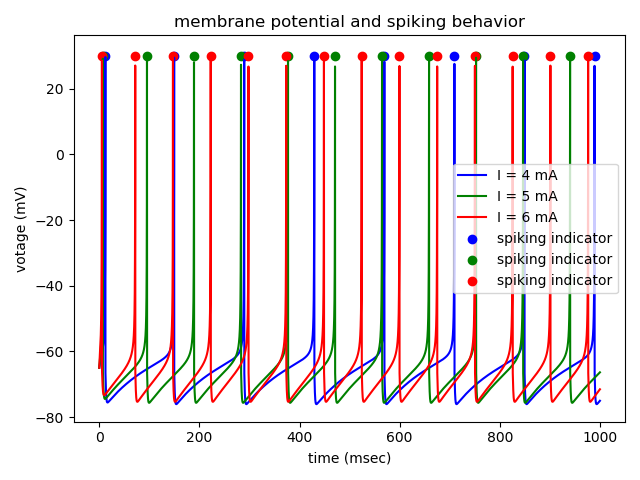
\includegraphics[scale=0.3]{plot_programming_4.png}}
			\subfigure[Hodgkin-Huxley]{
			\label{fig:Fig3.sub.H-H}
			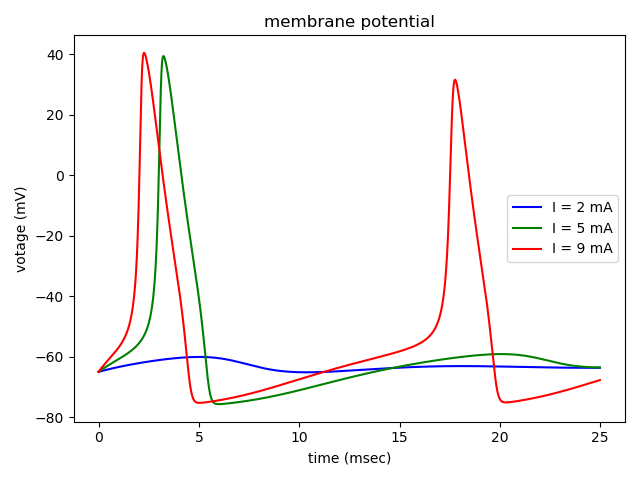
\includegraphics[scale=0.3]{plot_programming_5.png}}
			\caption{Izhikevich and Hodgkin-Huxley}
		\end{figure}
		
		\item Assume that you administer a drug named TTX, which inhibits the sodium current. Simulate the effect that TTX would have on the neural firing. Do the same for another drug, pronase, which eliminated sodium inactivation.
		
		TTX:
		
		Because TTX will inhibit the sodium current, sodium particle can not enter or exit the neuron. This situation is equal to closing all the sodium channel. Therefore, we can set 0 for $g_{na}m^3h(V-V_na)$ to simulate the effect of TTX. See the green curve in \ref{fig:fig5}.
		
		Pronase:
		
		Pronase will eliminate the sodium inactivation, which means all inactivation gate will be open. So, we can fixed $h$ to 1 to simulate the effect. See the red curve in \ref{fig:fig5}.
		
		\begin{figure}[ht]
			\centering
			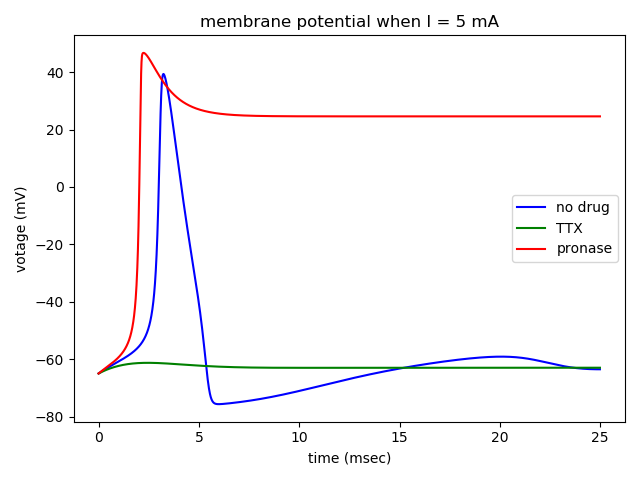
\includegraphics[scale=0.3]{plot_programming_6.png}
			\caption{TTX and pronase}
			\label{fig:fig5}
		\end{figure}
	\end{enumerate}
\end{document}